\chapter[METODOLOGI PENELITIAN]{METODOLOGI PENELITIAN}
\sloppy

Metodologi penelitian ini memaparkan tahapan sistematis yang dilakukan untuk mengevaluasi kinerja algoritma pelacakan multi-objek (\textit{Multi-Object Tracking}) dalam mengukur metrik perilaku konsumen pada lingkungan komersial beroklusi, serta menguji korelasi antara metrik standar akademik dan margin galat analitik bisnis di dunia nyata.

\section{Diagram Alir Penelitian}

Tahapan pelaksanaan penelitian dirancang secara terstruktur dan disajikan pada Gambar~\ref{fig:diagram_alir}.

\begin{figure}[htbp]
    \centering
    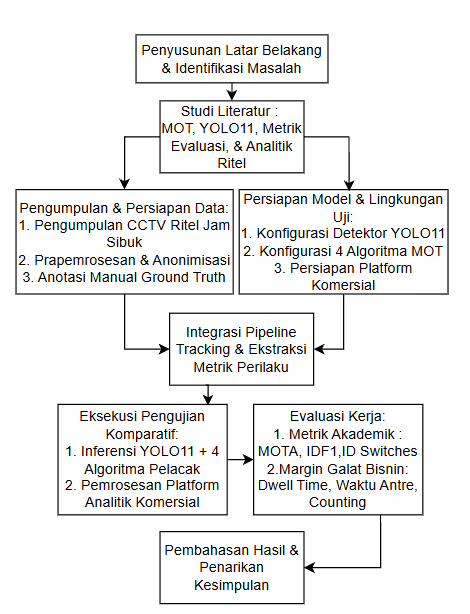
\includegraphics[width=0.75\textwidth, height=0.75\textheight, keepaspectratio]{gambar/diagramalir.png}
    \caption{Diagram Alir Penelitian}
    \label{fig:diagram_alir}
\end{figure}

Berdasarkan diagram alir pada Gambar~\ref{fig:diagram_alir}, tahapan penelitian diuraikan sebagai berikut:

\begin{enumerate}
    \item \textbf{Identifikasi Masalah}: Mengidentifikasi tantangan oklusi visual dan fenomena fragmentasi identitas (\textit{ID churn}) pada analitik video ritel komersial, serta merumuskan batasan masalah dan tujuan penelitian.
    \item \textbf{Studi Literatur}: Mengkaji landasan teoretis mengenai paradigma \textit{Tracking-by-Detection}, arsitektur YOLO11, algoritma pelacakan kontemporer (ByteTrack, BoT-SORT, OC-SORT, Deep OC-SORT), metrik evaluasi akademik (MOTA, IDF1), serta logika penghitungan metrik perilaku ritel.
    \item \textbf{Persiapan Data dan Ground Truth (Jalur Kiri)}: Mengumpulkan rekaman video CCTV dari dua lokasi area komersial pada jam sibuk, melakukan prapemrosesan dan anonimisasi data, serta menyusun anotasi manual (\textit{ground truth}) untuk lintasan objek dan waktu kejadian riil.
    \item \textbf{Persiapan Model dan Sistem (Jalur Kanan)}: Mengonfigurasi arsitektur pendeteksi objek YOLO11 sebagai variabel kontrol, menyiapkan modul inferensi untuk keempat algoritma pelacakan, serta menyiapkan akses terhadap platform analitik video komersial siap pakai sebagai pembanding industri.
    \item \textbf{Integrasi Pipeline dan Ekstraksi Metrik}: Mengintegrasikan modul deteksi, modul pelacakan, dan algoritma komputasi metrik perilaku (\textit{counting}, \textit{dwell time}, dan waktu antre) ke dalam satu alur pemrosesan data.
    \item \textbf{Eksekusi Pengujian Komparatif}: Menjalankan inferensi eksperimental terhadap rekaman video uji menggunakan keempat konfigurasi algoritma pelacakan serta memproses video yang sama melalui platform analitik komersial.
    \item \textbf{Evaluasi dan Analisis Korelasi Statistik}: Menghitung skor metrik pelacakan akademik (MOTA, IDF1, \textit{ID switches}), menghitung galat metrik perilaku terhadap data acuan manual (\textit{ground truth}), serta melakukan uji korelasi statistik antara keduanya.
    \item \textbf{Pembahasan dan Kesimpulan}: Menganalisis ketahanan masing-masing algoritma terhadap gangguan oklusi, menyimpulkan relevansi metrik akademik terhadap akurasi bisnis, dan menyusun laporan tugas akhir.
\end{enumerate}

\section{Pengumpulan Data dan Lingkungan Eksperimen}

Kualitas evaluasi empiris sangat bergantung pada representasi data uji terhadap kondisi dinamis di lapangan serta standarisasi lingkungan komputasi yang digunakan.

\subsection{Karakteristik Data Video Uji}
Data video yang digunakan dalam penelitian ini merupakan rekaman kamera pengawas (CCTV) yang diambil dari dua lokasi area komersial fisik yang berbeda (sektor ritel modern dan gerai F\&B). Pemilihan lokasi didasarkan pada variasi tata letak ruang, intensitas pergerakan pelanggan, serta tingkat kerapatan oklusi visual. Karakteristik dataset uji ditetapkan sebagai berikut:
\begin{enumerate}
    \item \textbf{Durasi dan Periode Perekaman}: Rekaman video diambil sepanjang 10--15 menit pada jam operasional sibuk (\textit{rush hour}), di mana interaksi antar-pelanggan dan penumpukan antrean mencapai intensitas tertinggi.
    \item \textbf{Sudut Pandang Kamera}: Kamera dipasang pada posisi elevasi sudut miring (\textit{elevated oblique view}) khas penempatan CCTV komersial, yang mencakup area etalase rak produk dan area antrean kasir.
    \item \textbf{Spesifikasi Teknis Video}: Video direkam pada resolusi standar \textit{High Definition} (1080p) dengan kecepatan bingkai 25 hingga 30 bingkai per detik (\textit{frames per second} / FPS).
    \item \textbf{Privasi dan Anonimisasi Data}: Demi menjaga privasi pengunjung, seluruh data video diproses secara anonim tanpa penerapan teknologi pengenalan biometrik wajah (\textit{facial recognition}). Analisis pergerakan murni didasarkan pada lokalisasi kotak pembatas tubuh manusia (kelas \textit{person}).
\end{enumerate}